%!TEX root = bare_conf.tex

\section{Evaluation}\label{sec:evaluation}


\begin{figure}[!t]
\centering
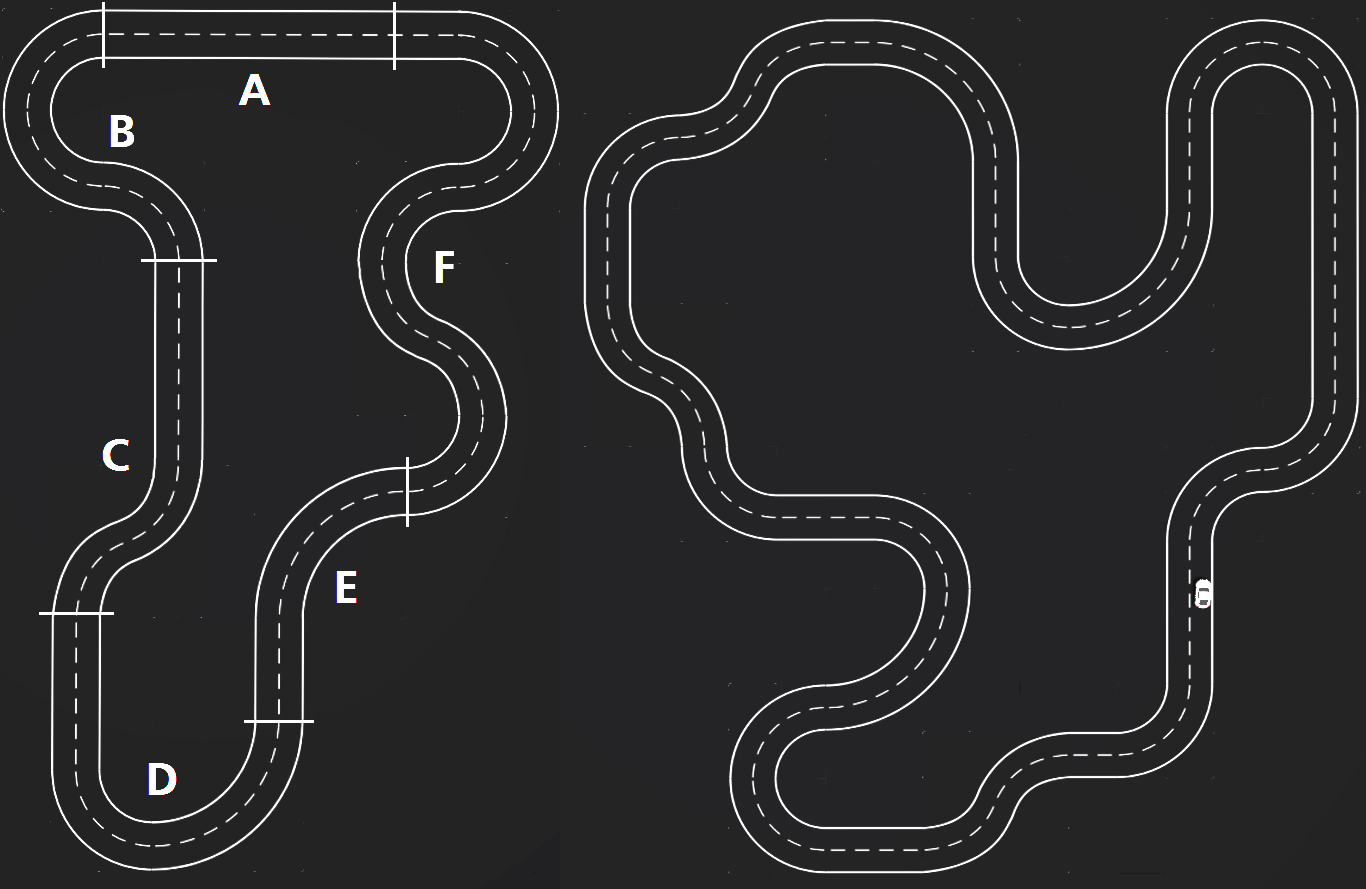
\includegraphics[scale=0.24]{../plots/track_both}
\caption{Left: Training track divided in six sections. Right: Additional test track with vehicle.}
\label{track}
\end{figure}

\begin{figure*}[!t]
\centering
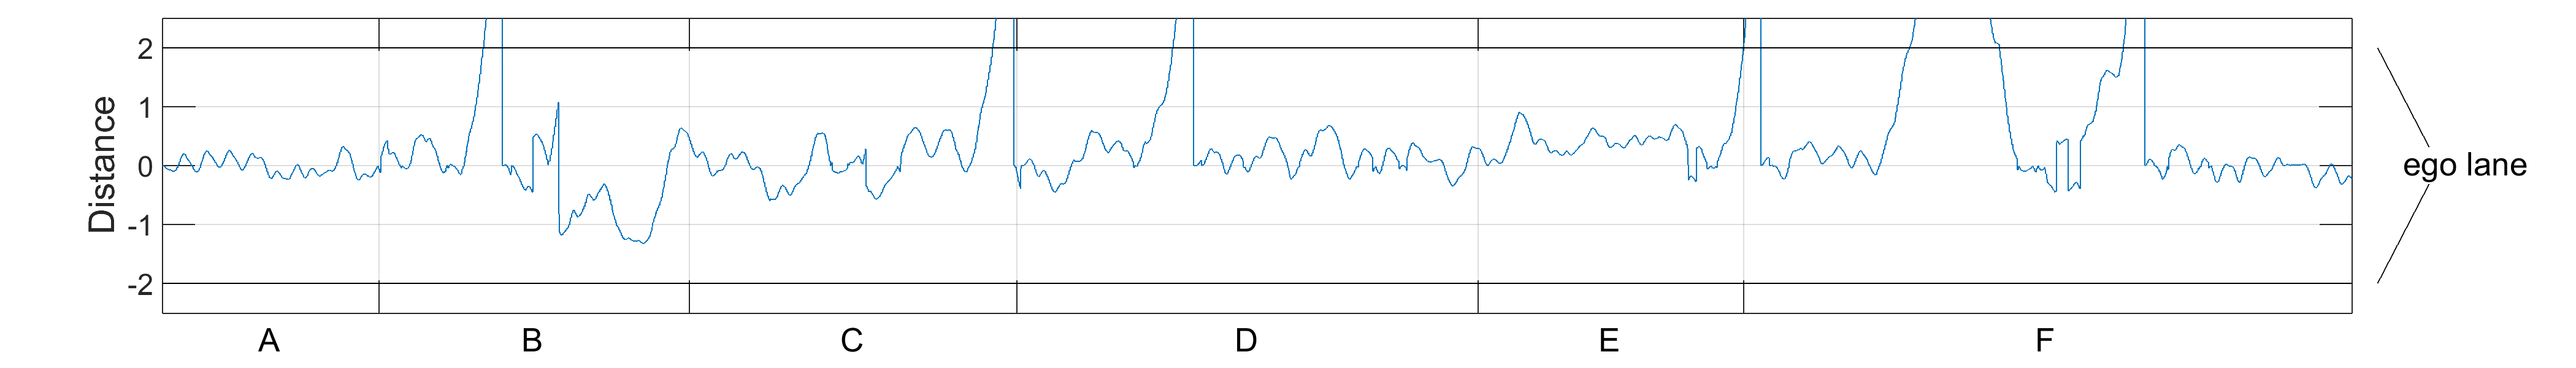
\includegraphics[scale=0.265]{../plots/dist_eval_log_distance_serpentine_06speed}
\vspace{0.5em}
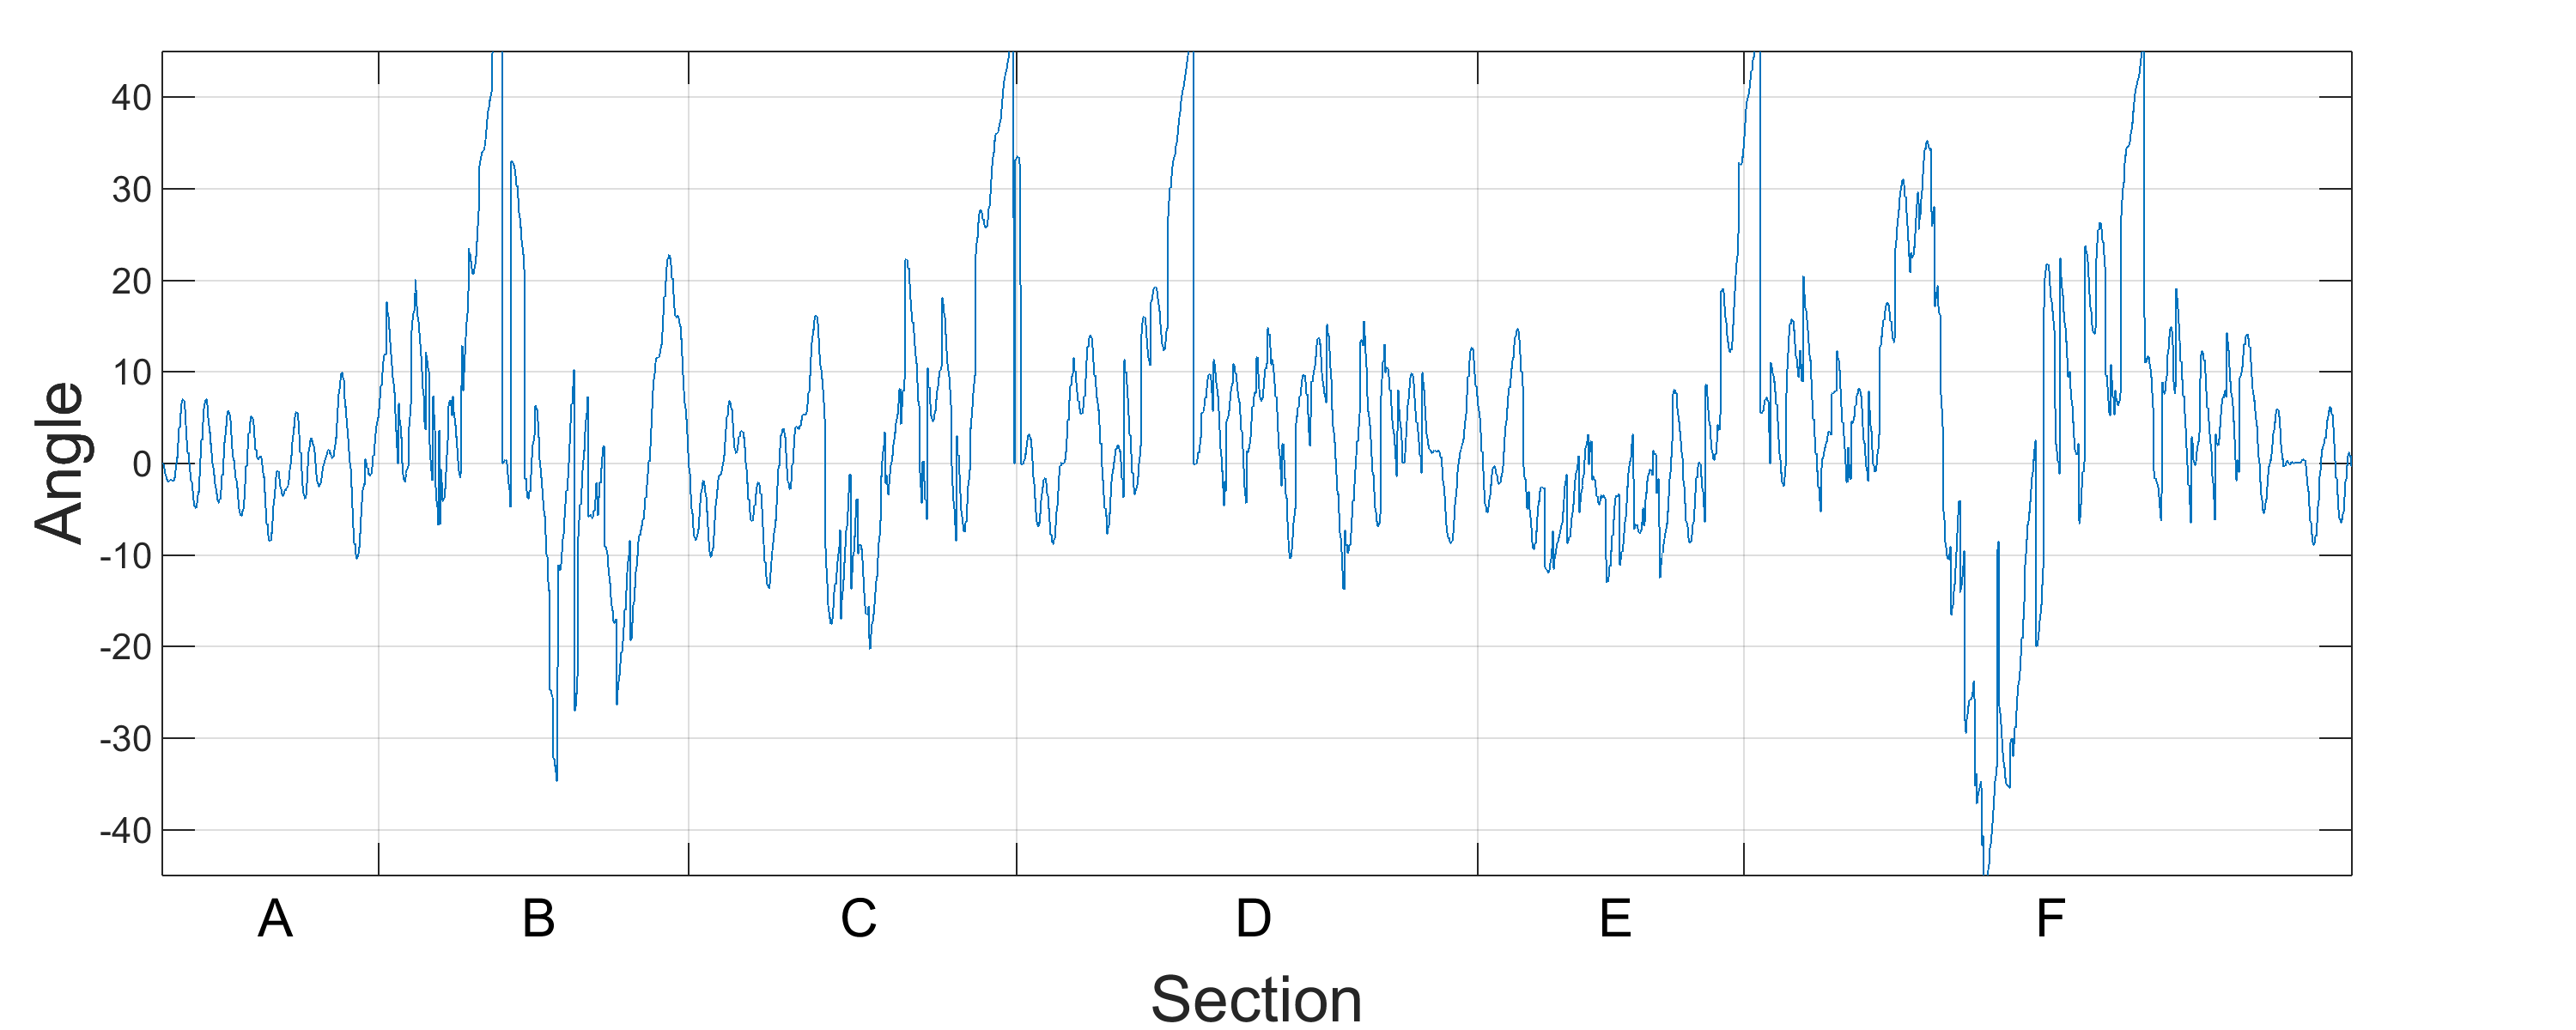
\includegraphics[scale=0.265]{../plots/ang_eval_log_distance_serpentine_06speed}
\vspace{-2.25em}
\caption{Distance-only approach. Distance in meters, angle in degrees.}
\label{distance06}
\vspace{1em}
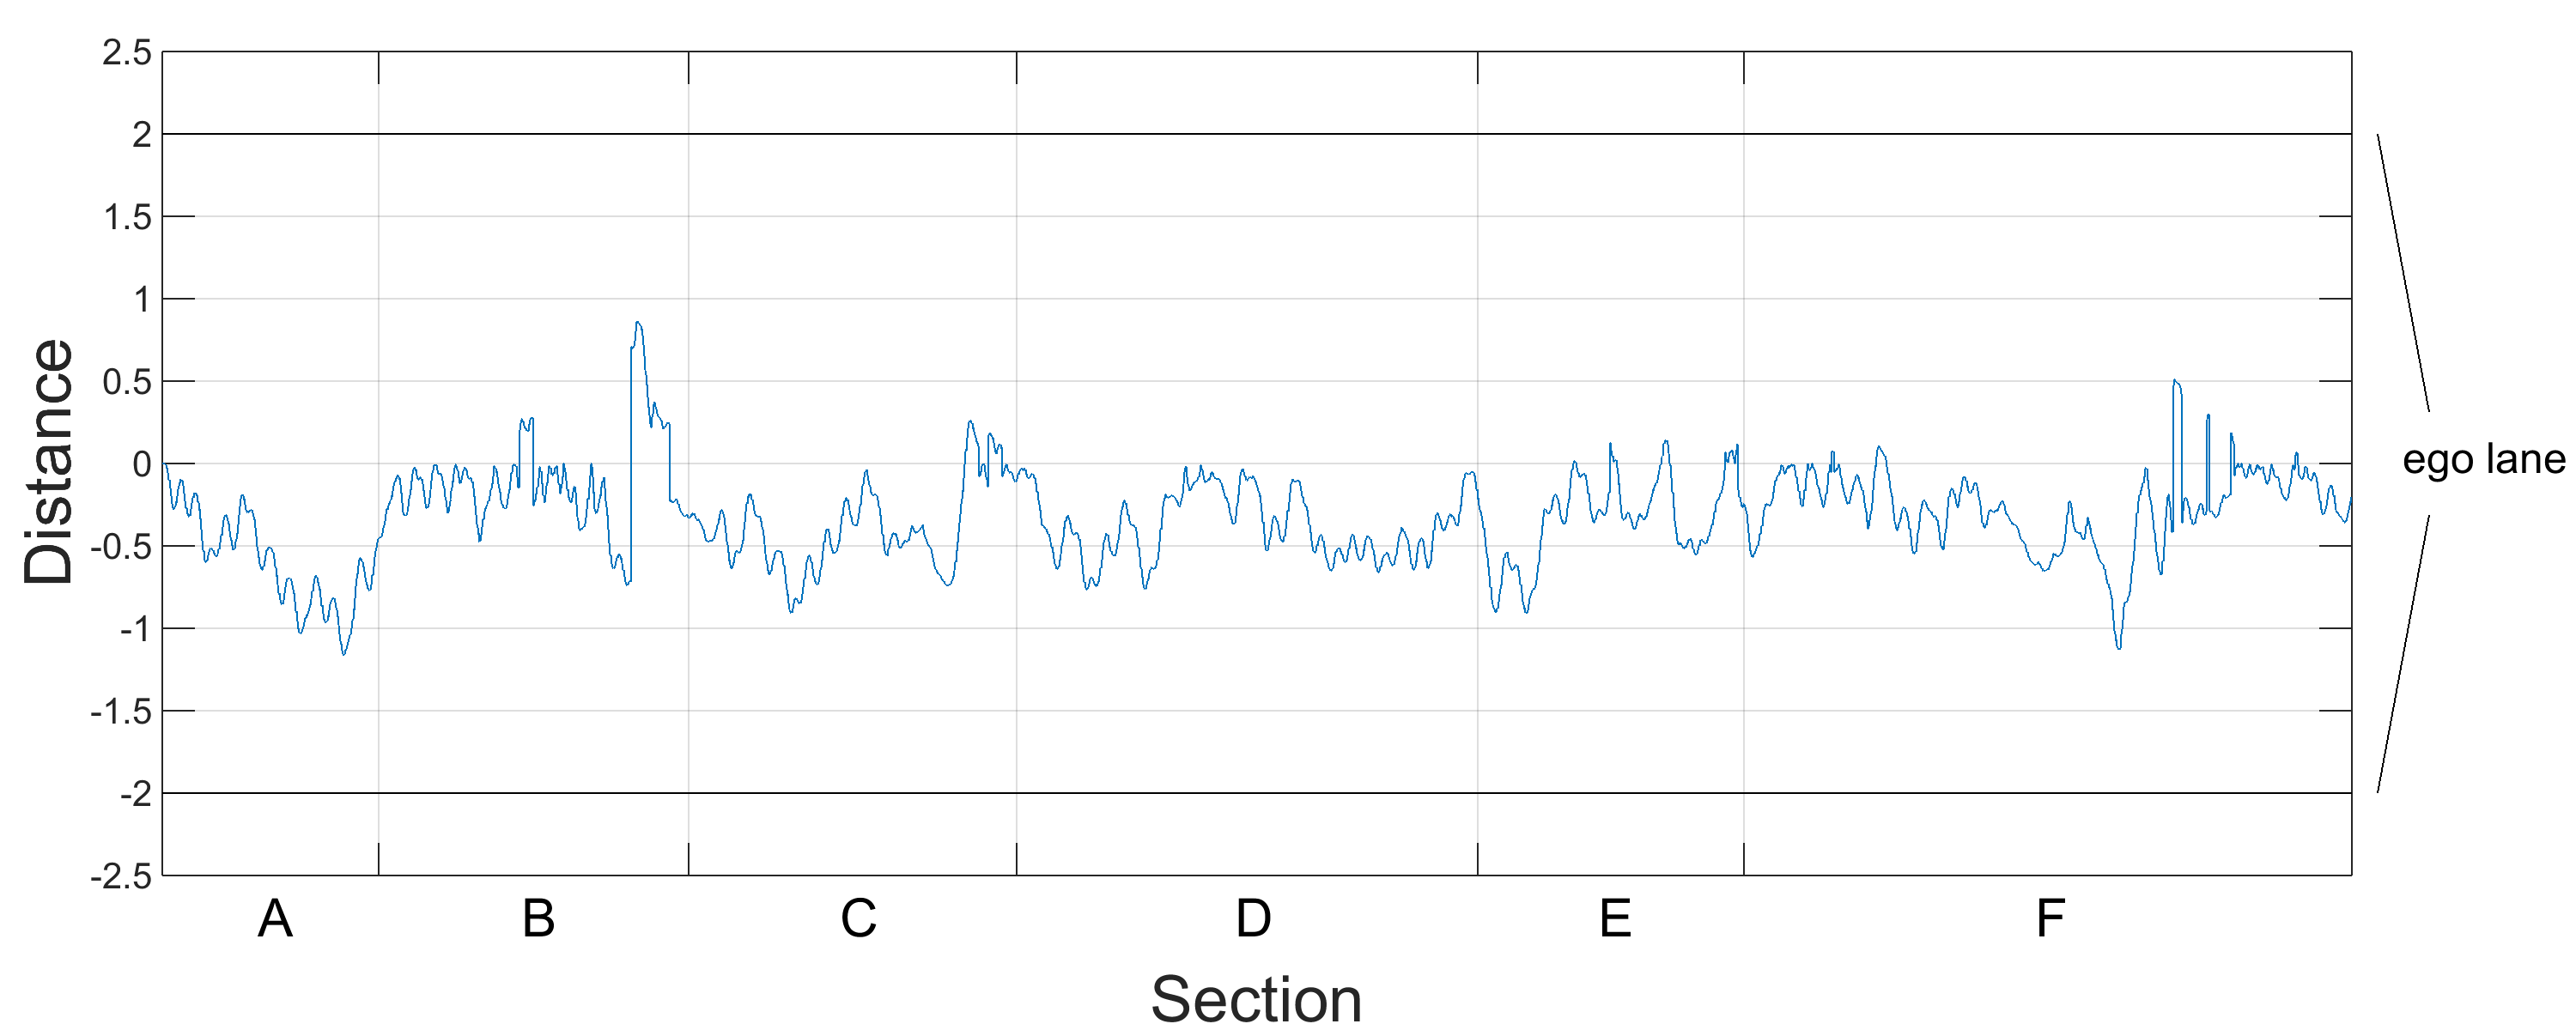
\includegraphics[scale=0.265]{../plots/dist_eval_log_dumb_actions_serpentine_06speed}
\vspace{0.5em}
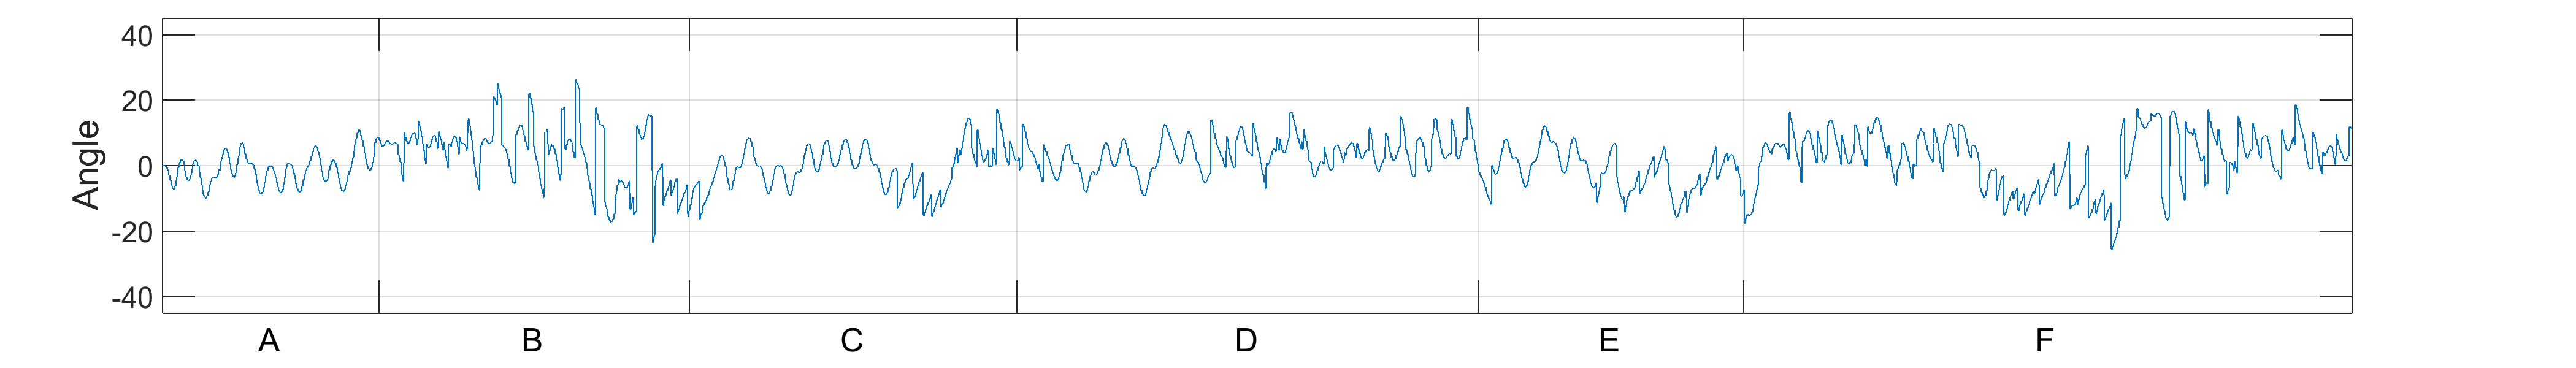
\includegraphics[scale=0.265]{../plots/ang_eval_log_dumb_actions_serpentine_06speed}
\vspace{-2.25em}\label{fig_first_case}
\caption{First action punishment added. Distance in meters, angle in degrees.}
\label{dumbactions06}
\end{figure*}

\begin{figure*}[!t]
\centering
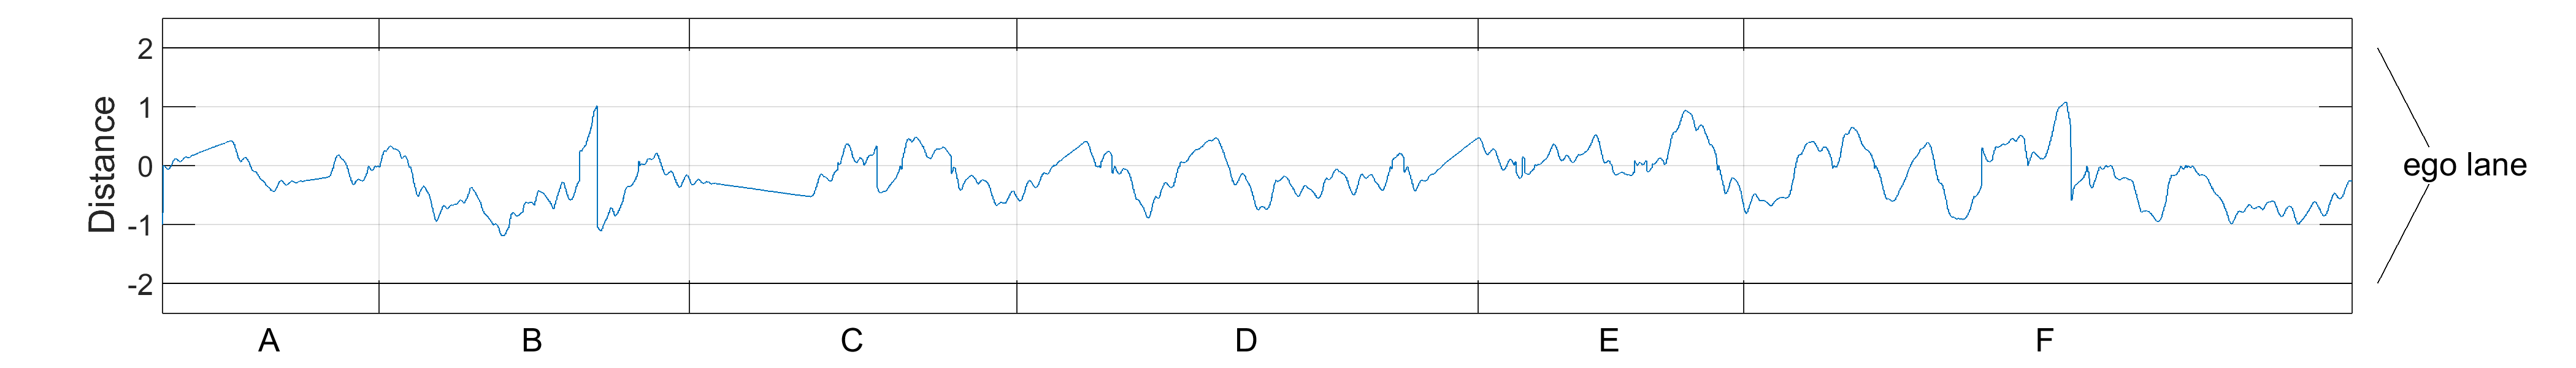
\includegraphics[scale=0.265]{../plots/dist_eval_log_straight_serpentine_06speed}
\vspace{0.5em}
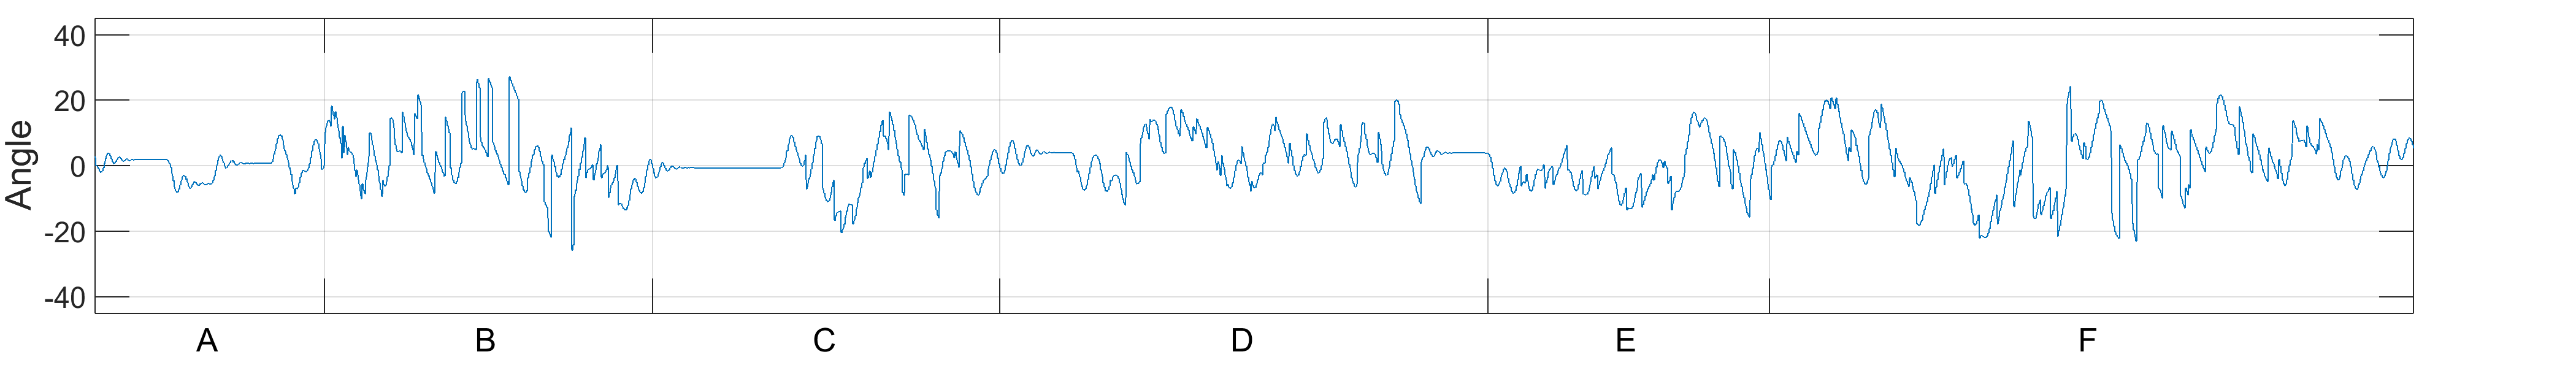
\includegraphics[scale=0.265]{../plots/ang_eval_log_straight_serpentine_06speed}
\vspace{-2.25em}
\caption{Straight action reward added. Distance in meters, angle in degrees.}
\label{straight06}
\vspace{1em}
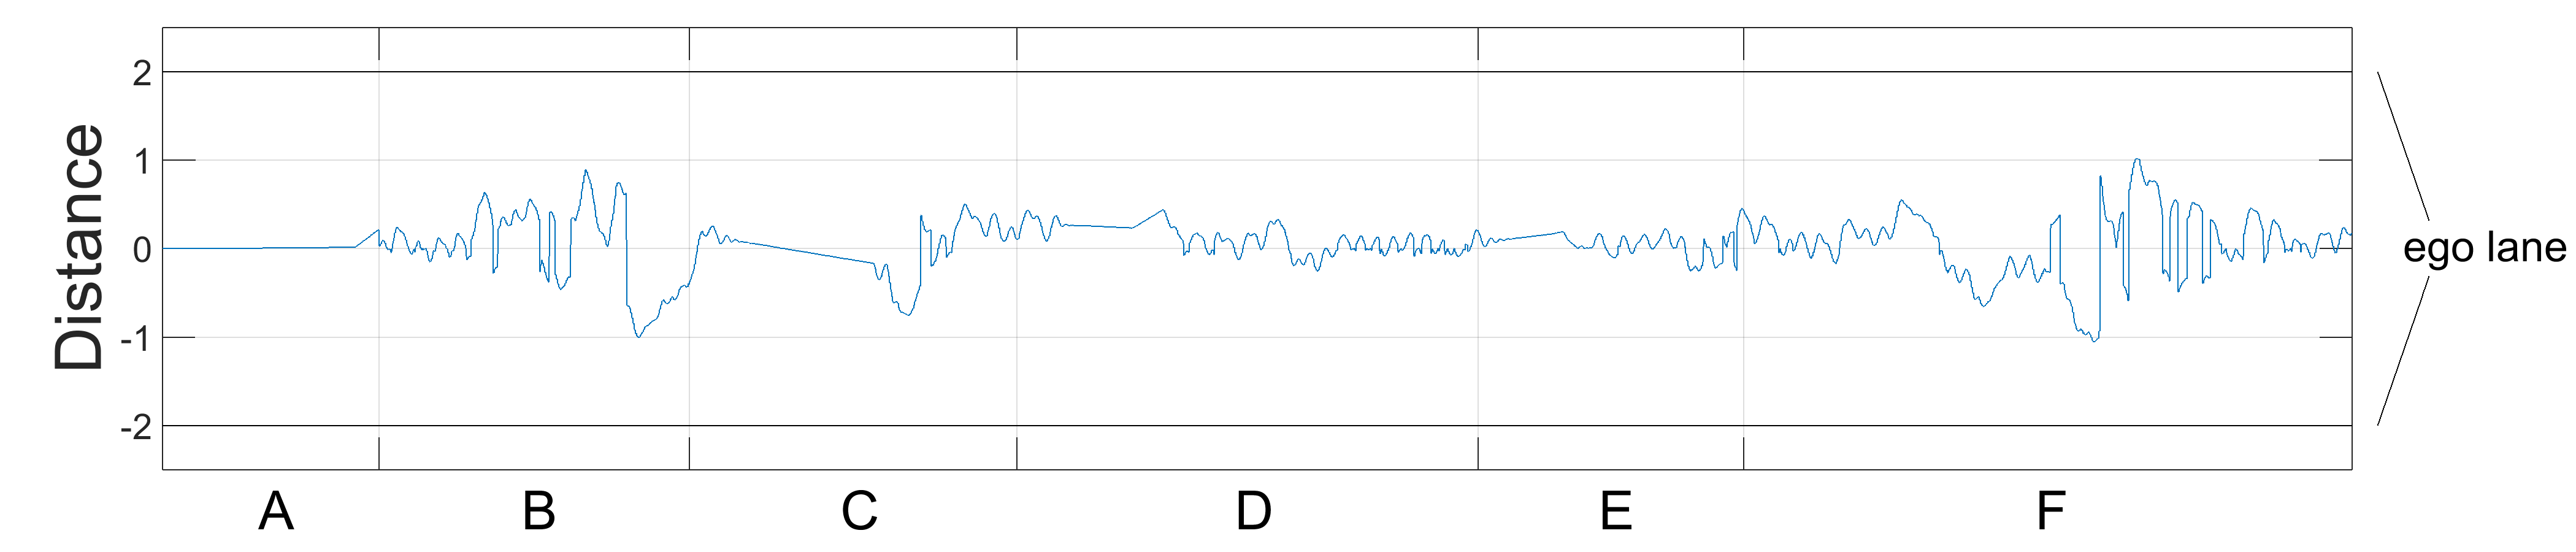
\includegraphics[scale=0.265]{../plots/dist_eval_log_smooth_serpentine_06speed}
\vspace{0.5em}
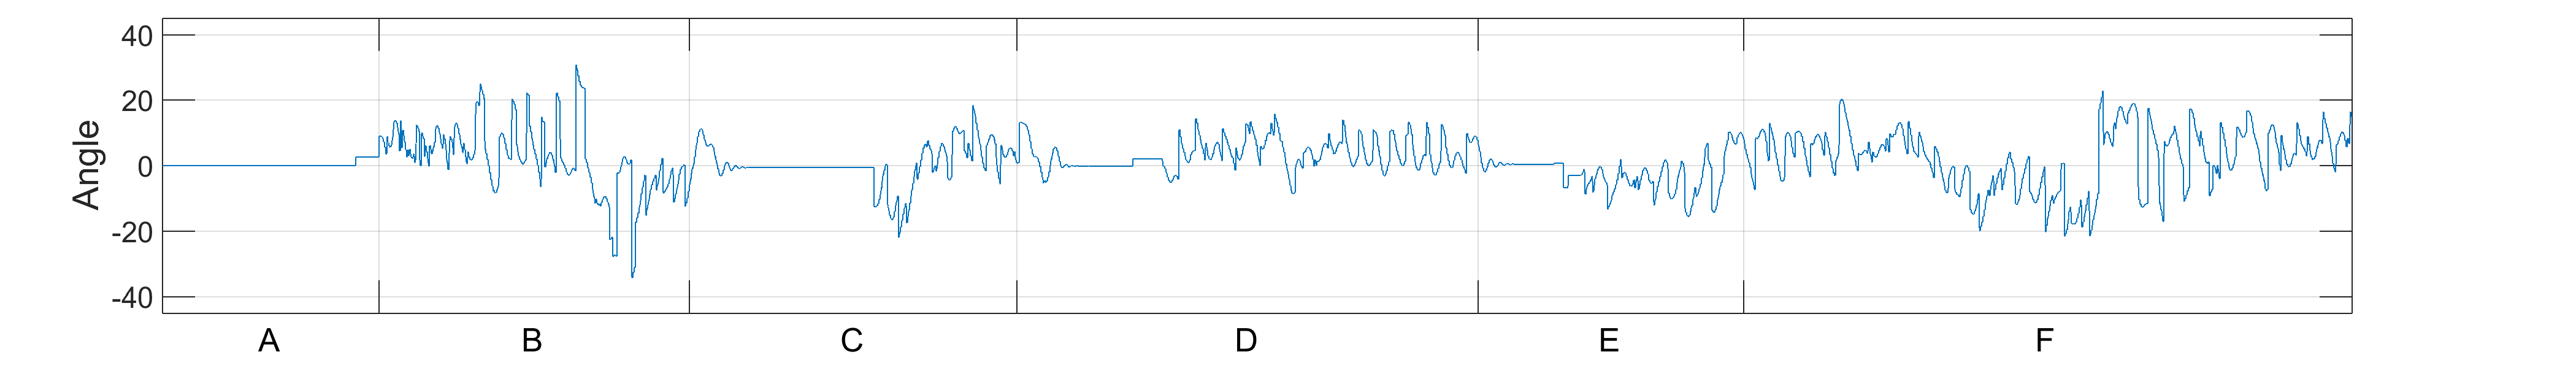
\includegraphics[scale=0.265]{../plots/ang_eval_log_smooth_serpentine_06speed}
\vspace{-2.25em}\label{fig_first_case}
\caption{Countersteering in curves punished. Distance in meters, angle in degrees.}
\label{smooth06}
\end{figure*}

\begin{figure*}[!t]
\centering
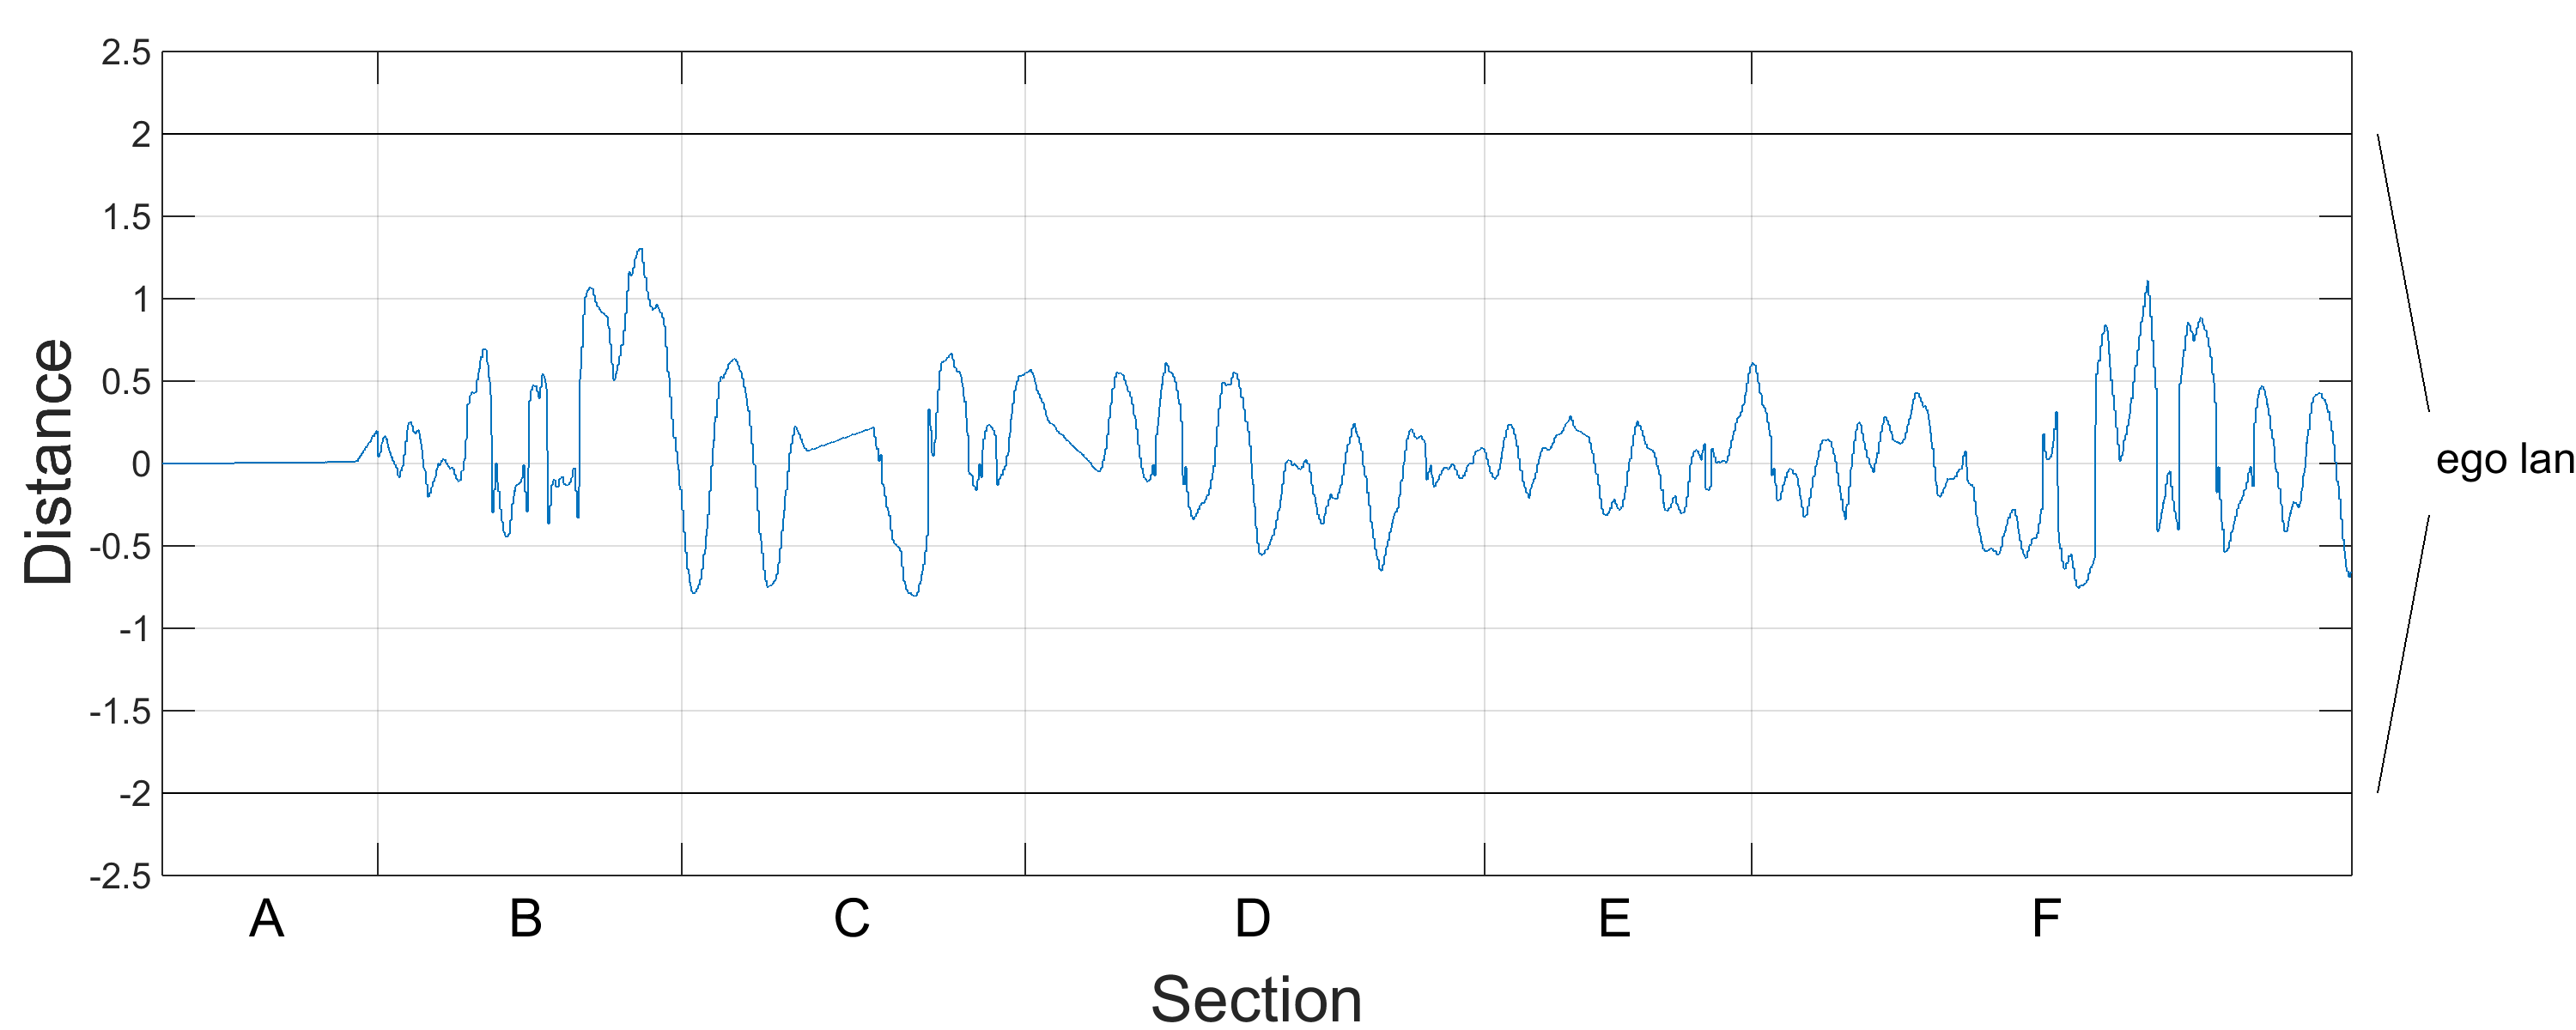
\includegraphics[scale=0.265]{../plots/dist_eval_log_smooth_serpentine_10speed}
\vspace{0.5em}
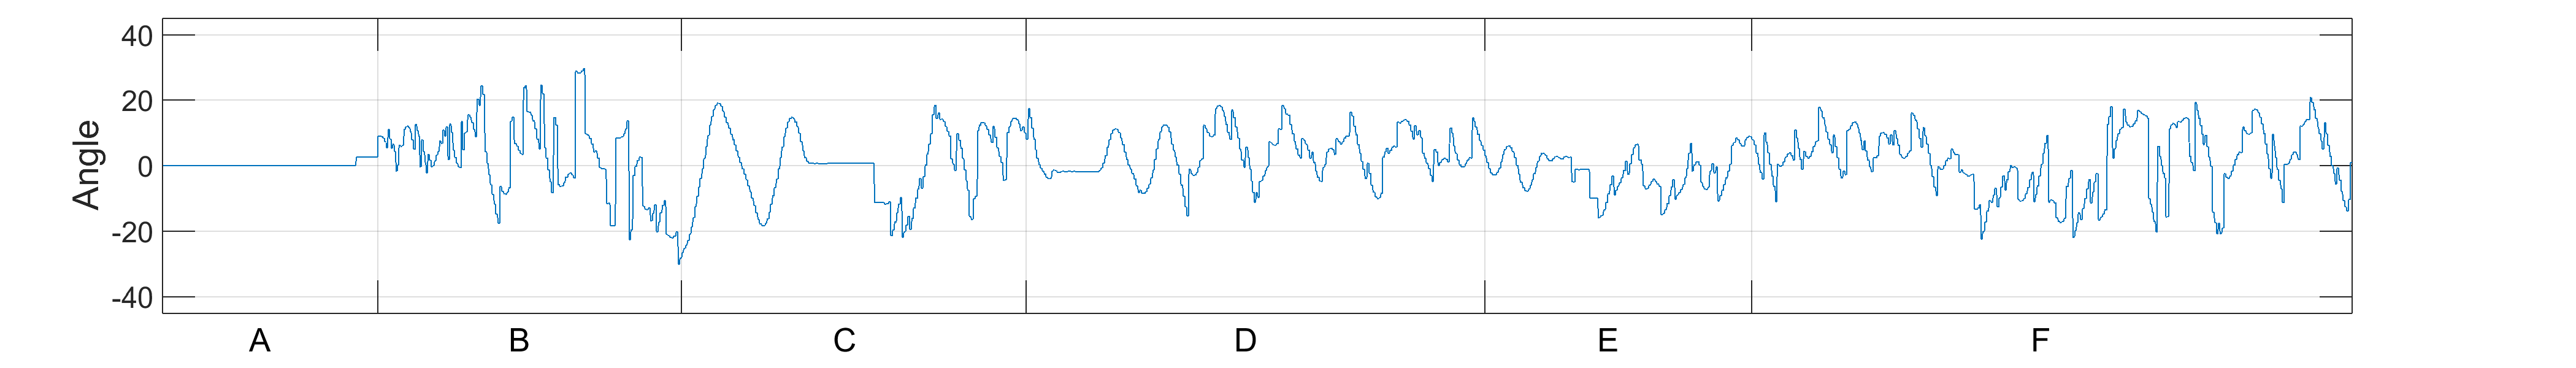
\includegraphics[scale=0.265]{../plots/ang_eval_log_smooth_serpentine_10speed}
\vspace{-2.25em}
\caption{Speed increased. Distance in meters, angle in degrees.}
\label{straight06}
\vspace{1em}
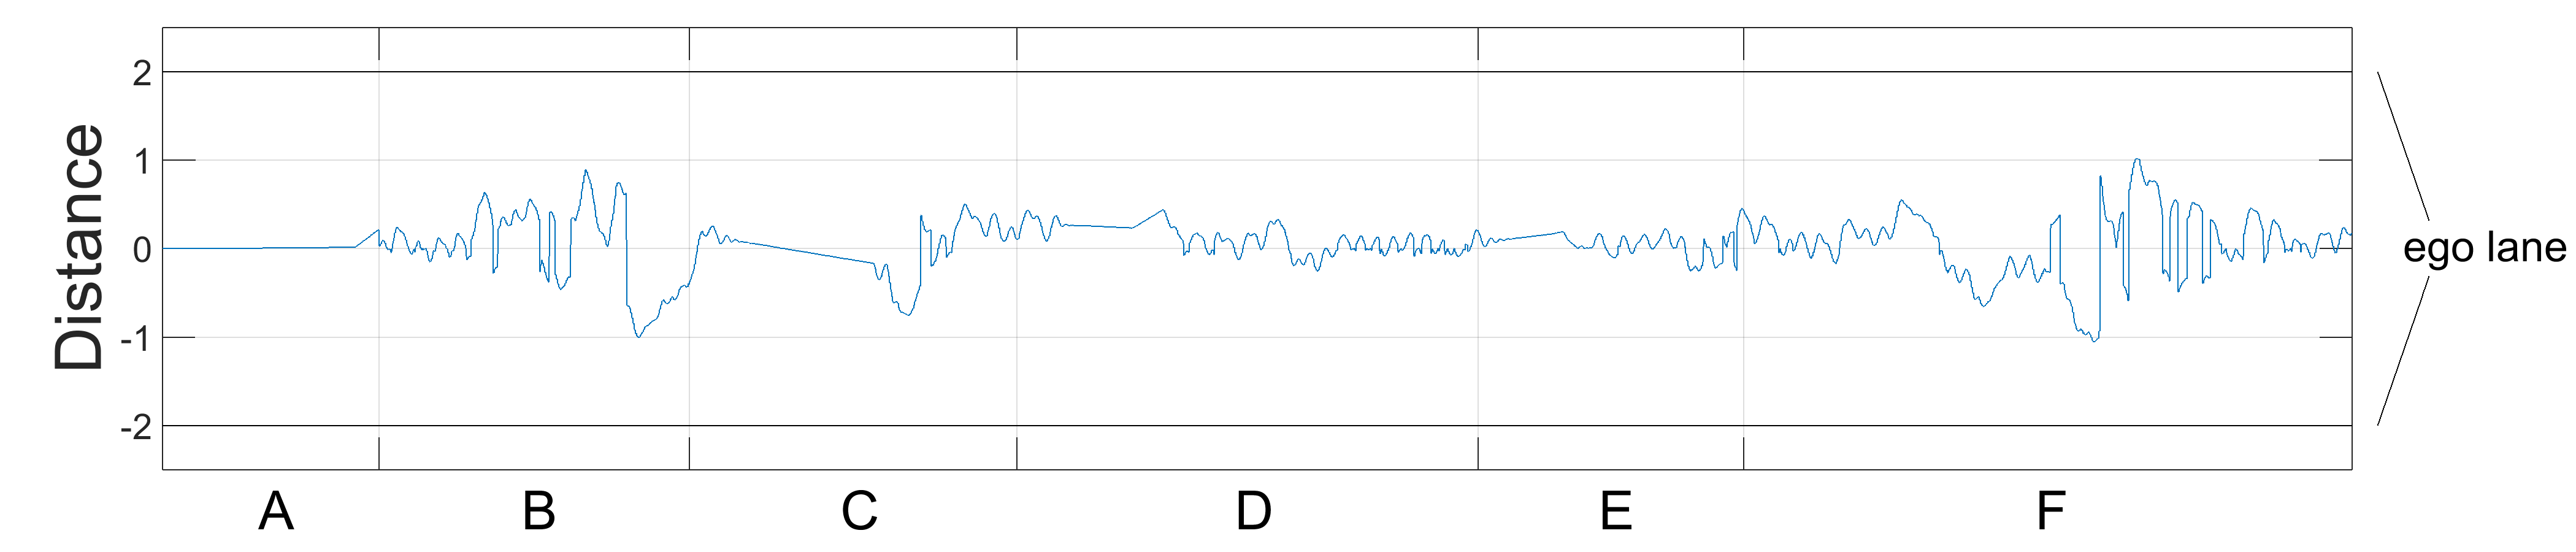
\includegraphics[scale=0.265]{../plots/dist_eval_log_smooth_serpentine_06speed}
\vspace{0.5em}
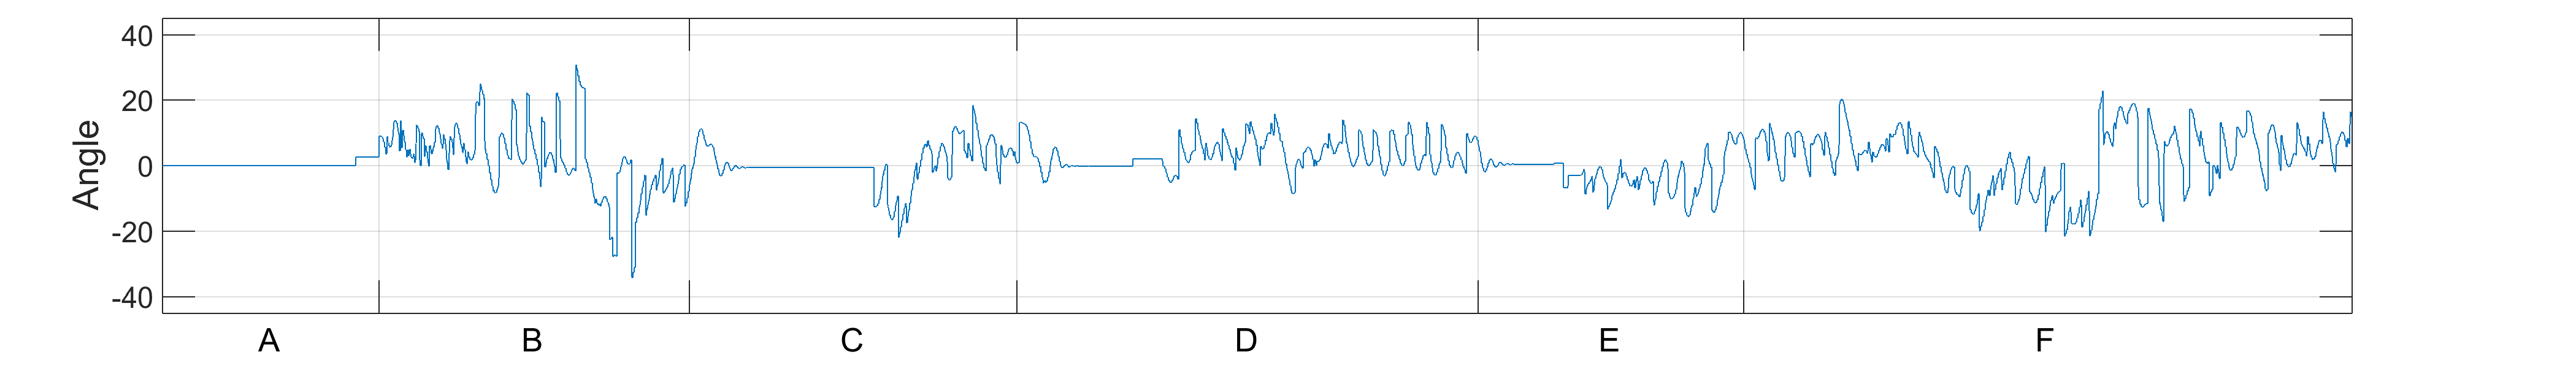
\includegraphics[scale=0.265]{../plots/ang_eval_log_smooth_serpentine_06speed}
\vspace{-2.25em}\label{fig_first_case}
\caption{Test on another track (see figure \ref{track}). Distance in meters, angle in degrees.}
\label{smooth06}
\end{figure*}

To evaluate each modification made to our reward function, we plotted distance and angle of the car in relation to the middle of the lane, as these are straightforward indicators for the quality of an approach. These plots were created for one lap on the same track, which was partitioned in several intervals for better comprehension of specific behaviour. The track and the sectors are displayed in figure \ref{track}, we will refer to these sectors in the following. For the distance plots we added lines indicating the designated lane to drive in. All plots are based on a vehicle, which was trained for at least 6 million iterations, meaning the training did already converge and no more noteworthy changes would occur. 

Figure \ref{distance06} displays our first approach using nothing but a distance based reward. From the distance plot it becomes obvious that this approach was flawed. While the vehicle could handle straight sections like A and ones with wide curves as can be seen in the second half of D and most of E, it was not able to handle narrow curves at all. Whenever the car drove away too far from the road we had to reset it back on it's lane and continue from there. This is shown by the large spikes in the distance plot. One more interesting thing to note here is the wide, large spike in section F, where the car was not actually reset, but drove off the road at the end of the left turn, cut a corner and found back onto the road by chance. The fact that the car always drove off the road on the same side is mostly due to the longer narrow curves, which were more troublesome, being almost exclusively left turns. The only such right turn would have been in F but was skipped by the car as we just explained. 
The angle plot fits this same picture. Whenever the car drove off, the angle shows a large spike, because the car would leave a curve by driving straight or even turning in the wrong way. In section F we can again find our anomaly of the car cutting a corner, illustrated by the large negative spike.
Throughout the whole lap the distance and angle plot depict a very shaky behaviour, but it was obvious that the car understood it's task of staying in it's designated lane.

In section \ref{sec:approach} we explained our reasoning of adding an action based reward on top of the distance reward. The result of adding only the punishment for steering away from the road whilst already being located and turned away from it is displayed in figure \ref{dumbactions06}. The improvement over the distance-only based approach is immense. The vehicle was now able to finish the whole lap without leaving the road and being reset. Overall the maximum recorded absolute distance was roughly one meter, which is already a solid performance. The angle plot for the current approach still shows a high overall frequency, which made a lot of sense, since the reward was still heavily distance based and with the limited amount of actions at it's disposal, the car zigzagged around the center lane.

Since the car was now able to follow the lane as intended, we started focusing on the driving experience. However we ran into problems when it came to defining globally valid action reward rules, hence we decided to have some factors only applied on straight sectors and others only in curves. This made the design process for these reward rules a lot less convoluted. First we decided to tackle the behaviour on straight sections, by rewarding the straight action when the vehicle was already very close to the center. The results can be seen in figure \ref{straight06}. The overall change with this additional rule was obviously only limited to the behaviour on straight sectors, since it did not affect the reward in curves. The car now adjusts it's orientation as soon as it enters a straight section, performing minor adjustments after drifting slightly away from the center. Right at the start of A, the vehicle steered slightly to one direction and then drove straight resulting in a single correction half way through A to stay close to the center, followed by another straight part right to the end of A. The straight part of C was managed a lot better, due to better initial alignment after B. To a lesser extend the same can be discerned at the beginning and end of D.

As we were pleased with the results on straight sections we focused our attention towards behaviour in curves. We knew we could not achieve perfectly smooth behaviour in curves because the limited action set simply did not allow it. With just two angles to choose from per side, the car would have no choice but to make corrections by choosing the straight action or even exploiting countersteering. We decided to reduce the latter by punishing it in curves as the final action reward rule. The associated plots can be found in figure \ref{smooth06}. The distance plot shows vast improvements in almost all sections. In comparison to the last approach we can now see how the straight section A can be mastered by simply steering straight, because the vehicles starting orientation is already perfectly aligned with the road. Sections C through E and about half of F are almost perfectly centered with only very little disturbances. The angle plot reflects this image, but also adds some further information. The car now decides to steer less aggressively into a curve to avoid getting on the inner side, which would result in the need to countersteer to stay close to the center. It now switches between steering into the curve and steering straight. This improvement is more noticeable for wider curves like in D and E, because the straight action is less decremental in those. In B and F there are still some regions in which the vehicle did not improve as much in relation to the earlier approaches, these sectors contain narrow curves and sharp changes in direction. There are various possible reasons for this. First of all the input image contains a lot less information in tight curves because the front-facing camera only picks up very little information in one of the lower corners and in addition to that the action set might not offer the needed tools to handle these types of curves. So the initial setup might be at fault, but there is another possible cause of error. To determine the orientation of the road we use a low poly representation of the track, which means the reward function is based on this approximation. Therefore we  are actually teaching the car to drive in a piecewise linear style, which looks worse in tighter curves.

%-RMSE plots for distance and angle?
%-for different track

